\chapter{Case Study: Private Blockchain for Crowdfunding}
\label{chapter:case-study}

In this case study, we explore the implementation of a private blockchain for crowdfunding using the Cosmos SDK. This approach is particularly relevant in the current technological landscape, where blockchain technology significantly impacts various industries, offering innovative paradigms for secure, decentralized transactions and data management. Crowdfunding, a popular method for raising capital, stands to benefit greatly from the advantages offered by blockchain technology, such as enhanced transparency, security, and efficiency.

\subsection{Relevance and Objectives}
\label{subsec:relevance-objectives}
The objectives of this case study are as follows:
\begin{itemize}
    \item To demonstrate the practical application of blockchain technology in a crowdfunding context, underscoring the advantages over traditional methods.
    \item To delve into the specific features and capabilities of the Cosmos SDK in constructing a customized, efficient, and secure private blockchain.
    \item To provide a comprehensive guide and framework for developers and entrepreneurs aiming to utilize blockchain technology in crowdfunding or related fields.
\end{itemize}

This case study seeks to bridge theoretical concepts with practical application, offering a tangible example of how blockchain technology can be applied innovatively in real-world scenarios.
\subsection{Cosmos SDK in Crowdfunding}
\label{subsec:cosmos-sdk-in-crowdfunding}

Crowdfunding represents a unique application for blockchain technology, where the principles of decentralization, transparency, and security are paramount. Utilizing the Cosmos SDK for a private blockchain in a crowdfunding context offers several distinct advantages:

\begin{itemize}
    \item \textbf{Modularity:} The Cosmos SDK's modular structure enables the development of specialized functionalities tailored to crowdfunding needs. Modules for project listings, investor interactions, and fund management can be created, providing a comprehensive ecosystem for crowdfunding activities.
    \item \textbf{Interoperability:} A key feature of the Cosmos SDK is its ability to facilitate interoperability between different blockchain networks. This feature is crucial for a crowdfunding platform, as it allows the integration of diverse assets and broadens the scope for investments and investor participation.
    \item \textbf{Scalability:} The Cosmos SDK is designed to support scalable applications, which is essential for crowdfunding platforms expecting a high volume of transactions and interactions. Its underlying consensus mechanisms, such as Tendermint BFT, ensure that the platform can handle growth efficiently without compromising performance.
    \item \textbf{Customizability:} The SDK's flexible architecture allows for the creation of a customized user experience and specific features that cater to the unique requirements of crowdfunding, such as project validation, funding stages, and return distributions.
    \item \textbf{Security:} Ensuring the security of funds and transactions is critical in crowdfunding. The Cosmos SDK's security model, which includes features like role-based permissions and secure transaction handling, provides a robust foundation for building a trustworthy crowdfunding platform.
\end{itemize}

In the following sections, we will explore the implementation aspects of a crowdfunding platform using the Cosmos SDK, focusing on the design, development, and operation of key features in line with the requirements of crowdfunding activities.

\subsubsection{Project Setup and State Modeling}
\label{subsubsec:project-setup-and-state-modeling}

The initial phase in developing a crowdfunding platform with the Cosmos SDK involves setting up the project structure and modeling the state. This process lays the foundation for how the blockchain will manage and store data related to crowdfunding activities.

\paragraph{Defining the Data Model}
\label{par:defining-the-data-model}

In a crowdfunding context, the state of the blockchain must accurately represent the dynamic relationships and activities between various entities such as projects, investors, and funding stages. The Cosmos SDK's flexibility in defining the data model is crucial for capturing the multifaceted nature of crowdfunding projects. This flexibility allows for the creation of tailored entities that reflect the specific needs and structures inherent in crowdfunding platforms.

For instance, the `Project` entity encapsulates essential information about each crowdfunding initiative, including its identification, sponsorship details, financial targets, and current status. This comprehensive representation is crucial for tracking the progress and managing the lifecycle of crowdfunding projects.

The `Investor` entity models the stakeholders in a project, detailing their investment contributions and accrued benefits. By defining this entity, the platform can effectively manage investor relations, equity distribution, and profit sharing, which are core aspects of crowdfunding dynamics.

The `Stage` entity reflects the phased approach common in crowdfunding projects, where each stage represents a milestone or a specific funding goal. This modular approach to project development and funding allows for more granular management and tracking of the project's progress.

\begin{lstlisting}[language=go, caption={Protobuf Definitions for Project, Investor, and Stage}, label=lst:protobuf-definitions]
message Project {
  uint64 id = 1;
  string sponsor = 2;
  cosmos.base.v1beta1.Coin target = 3 [(gogoproto.nullable) = false];
  cosmos.base.v1beta1.Coin current = 4 [(gogoproto.nullable) = false];
  string state = 5;
  repeated Investor investors = 6;
  repeated Stage stages = 7;
}

message Investor {
  string address = 1;
  cosmos.base.v1beta1.Coin equity = 2 [(gogoproto.nullable) = false];
  int64 profit = 3;
}

message Stage {
  string name = 1;
  cosmos.base.v1beta1.Coin allocation = 2 [(gogoproto.nullable) = false];
}
\end{lstlisting}


By leveraging Protobuf for defining these data structures, the Cosmos SDK ensures consistency, efficiency, and the ability to evolve the data model as the platform grows. This approach not only enhances the blockchain's data integrity but also ensures that it can adapt to the changing needs of crowdfunding activities.

\paragraph{State Management}
\label{par:state-management}

State management is a core aspect of any blockchain application. In the context of crowdfunding, the state represents the current condition of all projects, investments, and transactions on the platform. The Cosmos SDK's multistore structure allows each module to manage its part of the state, leading to enhanced modularity and maintainability.

\begin{figure}[H]
    \centering
    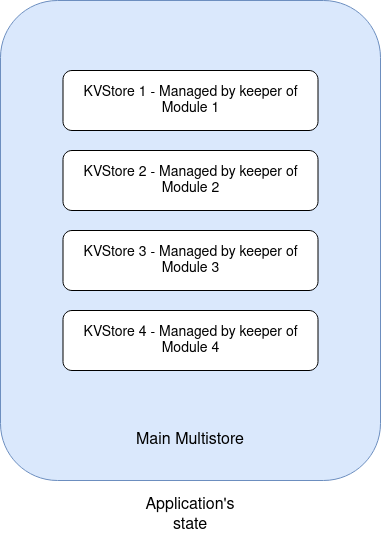
\includegraphics[scale=0.45]{figures/multistore.png}
    \caption{Application's state}
    \label{fig:application-multistore}
\end{figure}

\paragraph{Transaction Handling}
\label{par:transaction-handling}

Transactions in the crowdfunding platform are actions that change the state, such as creating a new project, investing in a project, or distributing funds. Each transaction type is defined with its validation logic, ensuring that only valid changes are applied to the state. The Cosmos SDK facilitates the creation of these transactions, handling the lifecycle from initiation to inclusion in the blockchain.

\paragraph{Query System}
\label{par:query-system}

A robust query system is essential for a crowdfunding platform, enabling users to retrieve information about projects and investments. The Cosmos SDK supports a flexible query interface, allowing users to interact with the blockchain's state efficiently. Queries can be made for specific projects, funding stages, and investment details, providing transparency and accessibility to platform participants.

In the next sections, we delve deeper into the implementation of these components, illustrating how the Cosmos SDK is utilized to build a comprehensive crowdfunding solution.

\section{Transaction Types and Their Implementation}
\label{sec:transaction-types-implementation}

In a crowdfunding platform developed with the Cosmos SDK, transactions play a pivotal role in facilitating various operations and interactions within the ecosystem. These transactions represent different actions that can be performed by users, such as creating new projects, investing in projects, or distributing returns. This section delves into the types of transactions that are fundamental to the crowdfunding platform and their implementation using the Cosmos SDK.

\subsection{Defining Transaction Types}
\label{subsec:defining-transaction-types}

The Cosmos SDK allows for the definition of custom transaction types to suit specific application needs. In the context of a crowdfunding platform, several transaction types are essential:

\begin{itemize}
    \item \textbf{CreateProject:} Initiates the creation of a new crowdfunding project, specifying details like project sponsor, funding target, and project stages.
    \item \textbf{InvestorBuyIn:} Enables investors to contribute funds to a project, marking their stake in the crowdfunding venture.
    \item \textbf{ChangeState:} Alters the state of a project, such as moving it from active to funded, or from funded to completed.
    \item \textbf{MoneyIn \& MoneyOut:} Manages the flow of funds into and out of the project, ensuring proper allocation and distribution.
    \item \textbf{SponsorCancel \& SponsorAccept:} Used by project sponsors to either cancel a project in its early stages or accept funding upon reaching the target.
    \item \textbf{AdminAdd \& AdminDelete:} Administering the platform by adding or removing administrators or project managers.
    \item \textbf{NextStage:} Progresses the project through its different stages, ensuring milestones are met before proceeding.
    \item \textbf{ShareProfit:} Distributes profits or returns to investors based on their contributions once the project generates revenue.
    \item \textbf{UpdateDraftProject:} Modifies details of a project that is still in its draft phase.
\end{itemize}

Each of these transaction types is implemented as a specific gRPC endpoint, as shown in Listing \ref{lst:gRPC-endpoints}. This structure not only brings clarity to the various operations possible within the crowdfunding platform but also ensures that each transaction is handled efficiently and securely within the Cosmos SDK framework.

The combination of well-defined transactions and efficient gRPC endpoints enables the crowdfunding platform to function seamlessly, providing a robust and user-friendly experience for both project creators and investors. This approach exemplifies the Cosmos SDK's versatility in handling diverse transaction types, a critical aspect for the success of any blockchain-based application.

\begin{lstlisting}[language=go, caption=gRPC endpoints definition,label={lst:gRPC-endpoints}]
service Msg {
  rpc CreateProject(MsgCreateProject) returns (MsgCreateProjectResponse);
  rpc InvestorBuyIn(MsgInvestorBuyIn) returns (MsgInvestorBuyInResponse);
  rpc ChangeState(MsgChangeState) returns (MsgChangeStateResponse);
  rpc MoneyIn(MsgMoneyIn) returns (MsgMoneyInResponse);
  rpc MoneyOut(MsgMoneyOut) returns (MsgMoneyOutResponse);
  rpc SponsorCancel(MsgSponsorCancel) returns (MsgSponsorCancelResponse);
  rpc SponsorAccept(MsgSponsorAccept) returns (MsgSponsorAcceptResponse);
  rpc AdminAdd(MsgAdminAdd) returns (MsgAdminAddResponse);
  rpc AdminDelete(MsgAdminDelete) returns (MsgAdminDeleteResponse);
  rpc NextStage(MsgNextStage) returns (MsgNextStageResponse);
  rpc ShareProfit(MsgShareProfit) returns (MsgShareProfitResponse);
  rpc UpdateDraftProject(MsgUpdateDraftProject) returns (MsgUpdateDraftProjectResponse);
}
\end{lstlisting}

\subsubsection{General Process for Implementing Transactions in Cosmos SDK}
\label{subsubsec:general-transaction-implementation}

The Cosmos SDK offers a structured approach to implementing transactions, which is crucial for maintaining the integrity and functionality of a blockchain application. The general process can be outlined in the following steps:

\begin{enumerate}
    \item \textbf{Defining the Transaction Message:}
    \begin{itemize}
        \item The first step is to define the transaction message using Protobuf. This involves specifying the structure of the data that will be included in the transaction. 
        \item The message should encompass all the necessary fields that are required to perform the transaction. This could include identifiers, amounts, addresses, or any other relevant information.
        \item The defined message acts as a blueprint for the transaction, ensuring that all necessary data is included and structured correctly for processing.
    \end{itemize}

    \item \textbf{Implementing the CLI Command:}
    \begin{itemize}
        \item Once the transaction message is defined, the next step is to implement the corresponding \gls{cli} command.
        \item This command allows users to interact with the blockchain application and execute transactions from the command line.
        \item The implementation involves coding the logic that will take user inputs, validate them, and construct the transaction message based on these inputs.
        \item The \gls{cli} command typically includes error handling and may have additional logic for transaction fees, signing, and broadcasting the transaction to the network.
    \end{itemize}
\newpage
    \item \textbf{Coding the Keeper Function:}
    \begin{itemize}
        \item The keeper function is responsible for updating the state of the blockchain based on the transaction.
        \item It involves writing the logic that will be executed when a transaction is processed. This includes validating the transaction, updating the state, and handling any side effects.
        \item The keeper function interacts with the blockchain's state machine, ensuring that the state changes are consistent and secure.
        \item It's crucial that the keeper function is thoroughly tested to ensure it handles all possible scenarios and edge cases correctly.
    \end{itemize}
\end{enumerate}

Following this structured process ensures that each transaction type is correctly implemented and integrated into the blockchain application. This methodology not only maintains the consistency and reliability of the application but also provides a clear framework for developing new transaction types as the application evolves.

In the following sections, we will be implementing different transaction, providing detailed insights into each step of the process for a comprehensive understanding.

\subsection{Implementation of the CreateProject Transaction}
\label{subsec:implementation-createproject}

The `CreateProject` transaction plays a pivotal role in the crowdfunding platform, enabling the initiation of new projects. Its implementation in the Cosmos SDK involves a series of well-defined steps, each contributing to the robust functionality of the transaction. This section details the engineering process behind the `CreateProject` transaction.

\subsubsection{Defining the Protobuf Message}
\label{subsubsec:protobuf-createproject}

The first step in implementing the `CreateProject` transaction is defining its structure using Protocol Buffers (Protobuf). Protobuf is a language-neutral, platform-neutral, extensible way of serializing structured data, making it ideal for this purpose.

\newpage
\begin{lstlisting}[language=go, caption=CreateProject protobuf definition, label={lst:create_project_proto}]
message MsgCreateProject {
  string                 sponsor = 1;
  cosmos.base.v1beta1.Coin target  = 2 [(gogoproto.nullable) = false];
  repeated Stage         stages  = 3;
}
\end{lstlisting}

The `MsgCreateProject` message encapsulates all necessary data for creating a project, such as the sponsor's name, target funding amount, and the project stages. Each field is carefully chosen to capture the essential attributes of a crowdfunding project.

\subsubsection{Implementing the CLI Command}
\label{subsubsec:cli-createproject}

The next phase involves implementing the \gls{cli} command. This command facilitates interaction with the blockchain, allowing users to initiate a `CreateProject` transaction.

The \gls{cli} command, as shown is Lst~\ref{lst:create-project-cli-implementation}, provides a user-friendly way to submit the `CreateProject` transaction. It includes error checking and handles user inputs, converting them into the Protobuf message format.

\newpage
\begin{lstlisting}[language=go, caption=CreateProject CLI protobuf definition, label={lst:create-project-cli-implementation}]
func CmdCreateProject() *cobra.Command {
	cmd := &cobra.Command{
		Use:   "create-project [target] [stages]",
		Short: "Broadcast message create-project",
		Args:  cobra.ExactArgs(2),
		RunE: func(cmd *cobra.Command, args []string) (err error) {
			argTarget, err := sdk.ParseCoinNormalized(args[0])
			if err != nil {
				return err
			}
			argStages, err := types.ParseStageNormalized(args[1])
			if err != nil {
				return err
			}
			clientCtx, err := client.GetClientTxContext(cmd)
			if err != nil {
				return err
			}
			msg := types.NewMsgCreateProject(
				clientCtx.GetFromAddress().String(),
				argTarget,
				argStages,
			)
			if err := msg.ValidateBasic(); err != nil {
				return err
			}
			return tx.GenerateOrBroadcastTxCLI(clientCtx, cmd.Flags(), msg)
		},
	}
	flags.AddTxFlagsToCmd(cmd)
	return cmd
}
\end{lstlisting}

\subsubsection{Backend Processing}
\label{subsubsec:backend-createproject}

Upon receiving a `CreateProject` transaction request, either through the \gls{cli} or a gRPC call, the Cosmos SDK's backend processes it. The transaction message is first validated, ensuring all required fields are provided and meet the necessary criteria.

\begin{verbatim}
$ daemonNamed tx appName create-project --sponsor "Project Sponsor" \
    --target "1000TOKENNAME" \
    --stages "Stage 1:100TOKENNAME,Stage 2:500TOKENNAME"
\end{verbatim}

This command, as illustrated, is an example of how users can initiate the `CreateProject` transaction using the Cosmos SDK CLI.

\subsubsection{Keeper Function Implementation}
\label{subsubsec:keeper-createproject}

The keeper function is where the transaction's logic is executed. This function updates the state of the blockchain with the new project's information.

\begin{lstlisting}[language=go, caption=Keeper implementation for CreateProject, label={lst:keeper_create_project}]
func (k msgServer) CreateProject(goCtx context.Context, msg *types.MsgCreateProject) (*types.MsgCreateProjectResponse, error) {
	ctx := sdk.UnwrapSDKContext(goCtx)
	var project = types.Project{
		Stages:  msg.Stages,
		Sponsor: msg.Sponsor,
		Target:  msg.Target,
	}
	id, err := k.AppendProject(
		ctx,
		project,
	)
	if err != nil {
		return &types.MsgCreateProjectResponse{}, err
	}
	types.EmitEvent(ctx, types.EventTypeProjectCreated, id, msg.Sponsor)
	return &types.MsgCreateProjectResponse{
		Id:      id,
		Address: msg.Sponsor,
	}, nil
}
\end{lstlisting}

The keeper function, as demonstrated, is responsible for appending the new project to the blockchain. It validates the transaction, checks for authorization, and updates the blockchain's state accordingly.

Following the successful creation of a project, an event is emitted. This event logs the creation, providing an auditable trail of the transaction. It includes details such as the project ID and sponsor's address.


\subsection{Updating Draft Projects}
\label{subsec:updating-draft-projects}

Projects in the crowdfunding platform, upon their initial creation, are in a \texttt{draft} state. This status indicates that the project details are preliminary and subject to revisions. The \texttt{UpdateDraftProject} transaction plays a crucial role in this phase, allowing authorized users to modify essential project attributes like target funding and project stages.

\subsubsection{Protobuf Message for UpdateDraftProject}
\label{subsubsec:protobuf-update-draft-project}

The structure of the \texttt{UpdateDraftProject} transaction is defined using Protobuf, ensuring a consistent and efficient data representation.

\newpage
\begin{lstlisting}[language=go, caption=UpdateDraftProject protobuf definition, label={lst:update_draft_project_proto}]
message MsgUpdateDraftProject {
  string                                creator   = 1;
  uint64                                projectId = 2;
  cosmos.base.v1beta1.Coin              target    = 4 [(gogoproto.nullable) = false];
  repeated Stage                        stages    = 5;
}
\end{lstlisting}

This Protobuf message includes fields for the project's unique identifier, updated target funding, and revised stages, capturing the essential elements for updating a draft project.

\subsubsection{Authorizing Updates}
\label{subsubsec:authorizing-updates}

Modification of a project's details requires appropriate authorization. The \texttt{UpdateDraftProject} transaction ensures that only authorized individuals, typically the project sponsor, can make changes to the project in its draft state.

\subsubsection{Implementing the Keeper Function}
\label{subsubsec:keeper-update-draft}

The keeper function is at the core of processing the \texttt{UpdateDraftProject} transaction. It validates the transaction, checks for authorization, and applies the updates to the project's state.

\begin{lstlisting}[language=go, caption=Keeper implementation for UpdateDraftProject, label={lst:keeper-update-draft}]
func (k msgServer) UpdateDraftProject(goCtx context.Context, msg *types.MsgUpdateDraftProject) (*types.MsgUpdateDraftProjectResponse, error) {
	ctx := sdk.UnwrapSDKContext(goCtx)
	projectId, err := k.updateDraftProjectInfo(ctx, msg.ProjectId, msg.Target, msg.Stages, msg.Creator)
	if err != nil {
		return nil, err
	}
	return &types.MsgUpdateDraftProjectResponse{
		ProjectId: projectId,
	}, nil
}
func (k Keeper) updateDraftProjectInfo(ctx sdk.Context, projectId uint64, target sdk.Coin, stages []*types.Stage, signer string) (uint64, error) {
	project, found := k.getProjectId(ctx, projectId)
	if !found {
		return 0, types.ErrProjectNotFound
	}
	if strings.Compare(signer, project.Sponsor) != 0 {
		return 0, types.ErrNotProjectSponsor
	}
	if strings.Compare(project.State, types.ProjectStateDraft) != 0 {
		return 0, types.ErrProjectNotDraft
	}
	if err := k.checkStages(stages, target); err != nil {
		return 0, err
	}
	project.Target = target
	project.Stages = stages
	k.saveProject(ctx, &project)
	return project.Id, nil
}
\end{lstlisting}

This keeper function checks if the project is in a draft state, validates the updates against the existing project structure, and then commits the changes to the blockchain.

\subsubsection{CLI Command for Updating Draft Projects}
\label{subsubsec:cli-update-draft}

To facilitate user interaction with the blockchain for updating projects, a \gls{cli} command is provided, simplifying the process of initiating the \texttt{UpdateDraftProject} transaction.

\newpage
\begin{lstlisting}[language=go, caption=Create Project CLI definition, label={lst:update-draft-cli}]
func CmdUpdateDraftProject() *cobra.Command {
	cmd := &cobra.Command{
		Use:   "update-draft-project [project-id] [target] [stages]",
		Short: "Broadcast message update-draft-project",
		Args:  cobra.ExactArgs(3),
		RunE: func(cmd *cobra.Command, args []string) (err error) {
			argProjectId, err := cast.ToUint64E(args[0])
			if err != nil {
				return err
			}
			argTarget, err := sdk.ParseCoinNormalized(args[1])
			if err != nil {
				return err
			}
			argStages, err := types.ParseStageNormalized(args[2])
			if err != nil {
				return err
			}
			clientCtx, err := client.GetClientTxContext(cmd)
			if err != nil {
				return err
			}
			msg := types.NewMsgUpdateDraftProject(
				clientCtx.GetFromAddress().String(),
				argProjectId,
				argTarget,
				argStages,
			)
			if err := msg.ValidateBasic(); err != nil {
				return err
			}
			return tx.GenerateOrBroadcastTxCLI(clientCtx, cmd.Flags(), msg)
		},
	}
	flags.AddTxFlagsToCmd(cmd)
	return cmd
}
\end{lstlisting}

This CLI command allows users to specify the project ID, updated target, and revised stages, streamlining the process of modifying a draft project.

\subsubsection{Executing the Transaction}
\label{subsubsec:executing-update-draft}

The execution of the \texttt{UpdateDraftProject} transaction can be done via the Cosmos SDK \gls{cli} or through a gRPC call. The CLI command example is as follows:

\begin{verbatim}
$ daemonNamed tx appName update-draft-project --project-id "idNumber" \
    --target "1000TOKENNAME" \
    --stages "Stage 1:100TOKENNAME,Stage 2:500TOKENNAME"
\end{verbatim}

This command line initiates the transaction, sending the updated project details to the blockchain for processing and validation.

The \texttt{UpdateDraftProject} transaction is an essential feature of the crowdfunding platform, offering flexibility and control during the project's initial development phase. It ensures that projects can evolve and refine their details before entering the active fundraising stage, thereby enhancing the platform's adaptability and responsiveness to changing needs and feedback.

\subsection{Investor Participation Transaction}
\label{subsec:investor-participation}

The \texttt{InvestorBuyIn} transaction is fundamental in the crowdfunding platform, enabling investors to financially contribute to projects of their interest. This transaction marks the investor's entry into the project, signifying their commitment and expectation of potential returns.

\subsubsection{Protobuf Message for InvestorBuyIn}
\label{subsubsec:protobuf-investor-buyin}

The transaction's structure is defined using Protobuf, which ensures a clear and efficient representation of the necessary data for an investor's participation.

\begin{lstlisting}[language=go, caption=InvestorBuyIn protobuf definition, label={lst:investor_buyin_proto}]
message MsgInvestorBuyIn {
  string                           investor = 1;
  uint64                           projectId = 2;
  cosmos.base.v1beta1.Coin         amount    = 3 [(gogoproto.nullable) = false];
}
\end{lstlisting}

This Protobuf message includes the investor's address, the project ID they wish to invest in, and the amount of their investment.

\subsubsection{Processing Investor Contributions}
\label{subsubsec:processing-investor-contributions}

Upon initiation of an \texttt{InvestorBuyIn} transaction, the platform processes the investor's contribution, ensuring that it adheres to the project's requirements and investment rules.

\subsubsection{Implementing the Keeper Function for InvestorBuyIn}
\label{subsubsec:keeper-investor-buyin}

The keeper function is responsible for validating and processing the \texttt{InvestorBuyIn} transaction, updating the project's state with the new investment details.

\begin{lstlisting}[language=go, caption=Keeper implementation for Investor Buy-in, label={lst:keeper_investor_buyin}]
func (k msgServer) InvestorBuyIn(goCtx context.Context, msg *types.MsgInvestorBuyIn) (*types.MsgInvestorBuyInResponse, error) {
	ctx := sdk.UnwrapSDKContext(goCtx)
	var investor = types.Investor{
		Address: msg.Investor,
		Equity:  msg.Amount,
	}
	appendedAddr, err := k.AppendInvestorBuyIn(ctx, msg.ProjectId, investor)
	if err != nil {
		return &types.MsgInvestorBuyInResponse{}, err
	}
	return &types.MsgInvestorBuyInResponse{
		InvestorAddr: appendedAddr,
	}, nil
}

func (k Keeper) AppendInvestorBuyIn(ctx sdk.Context, id uint64, investor types.Investor) (string, error) {
	if investor.Equity.Amount.Equal(sdk.ZeroInt()) {
		return "", types.ErrCoinZeroAmount
	}
	project, found := k.getProjectId(ctx, id)
	if !found {
		return "", types.ErrProjectNotFound
	}
	if project.State != types.ProjectStateActive {
		return "", types.ErrProjectNotActive
	}
	if strings.Compare(project.Target.Denom, investor.Equity.Denom) != 0 {
		return "", types.ErrCoinDiffDenom
	}
	if project.Target.Sub(project.Current).IsLT(investor.Equity) {
		return "", types.ErrOverFunded
	}
	addr, err := sdk.AccAddressFromBech32(investor.Address)
	if err != nil {
		return "", err
	}
	if err := k.bankKeeper.SendCoinsFromAccountToModule(ctx, addr, types.ModuleName, sdk.NewCoins(investor.Equity)); err != nil {
		return "", err
	}
	project.Investors = appendInvestor(project.Investors, &investor)
	project.Current = project.Current.Add(investor.Equity)
	if project.Target.IsEqual(project.Current) {
		project.State = types.ProjectStatePending
		types.EmitEvent(ctx, types.EventTypeProjectPending, project.Id, investor.Address)
	} else {
		types.EmitEvent(ctx, types.EventTypeProjectInvested, project.Id, investor.Address)
	}
	k.saveProject(ctx, &project)
	return investor.Address, nil
}
\end{lstlisting}

This function ensures that the investment is correctly recorded and allocated to the specified project, updating the project's current funding status and the investor's stake.

\subsubsection{CLI Command for Investor Participation}
\label{subsubsec:cli-investor-participation}

A \gls{cli} command is provided to facilitate the investor's interaction with the blockchain, enabling them to execute the \texttt{InvestorBuyIn} transaction seamlessly.

\begin{lstlisting}[language=go, caption=Investor Buy-in CLI Definition, label={lst:investor-buyin-cli}]
func CmdInvestorBuyIn() *cobra.Command {
	cmd := &cobra.Command{
		Use:   "investor-buy-in [project-id] [amount]",
		Short: "Broadcast message investor-buy-in",
		Args:  cobra.ExactArgs(2),
		RunE: func(cmd *cobra.Command, args []string) (err error) {
			argProjectId, err := cast.ToUint64E(args[0])
			if err != nil {
				return err
			}
			argAmount, err := sdk.ParseCoinNormalized(args[1])
			if err != nil {
				return err
			}
			clientCtx, err := client.GetClientTxContext(cmd)
			if err != nil {
				return err
			}
			msg := types.NewMsgInvestorBuyIn(
				clientCtx.GetFromAddress().String(),
				argProjectId,
				argAmount,
			)
			if err := msg.ValidateBasic(); err != nil {
				return err
			}
			return tx.GenerateOrBroadcastTxCLI(clientCtx, cmd.Flags(), msg)
		},
	}
	flags.AddTxFlagsToCmd(cmd)
	return cmd
}
\end{lstlisting}

Through this command, investors can specify the project they wish to invest in and the amount of their contribution, simplifying the investment process.

\subsubsection{Executing the InvestorBuyIn Transaction}
\label{subsubsec:executing-investor-buyin}

Investors can execute the \texttt{InvestorBuyIn} transaction via the Cosmos SDK \gls{cli} or through a gRPC request. The CLI command example is as follows:

\begin{verbatim}
$ daemonNamed tx appName investor-buy-in --project-id "projectId" \
    --amount "investmentAmount"
\end{verbatim}

This command facilitates the transaction process, marking the investor's financial entry into the selected project.

The \texttt{InvestorBuyIn} transaction plays a vital role in the crowdfunding ecosystem, enabling a direct and transparent channel for investors to support projects. It epitomizes the decentralized and participant-driven nature of blockchain-based crowdfunding, offering an efficient and secure mechanism for investment activities.

\subsection{Transitioning Project States}
\label{subsec:transitioning-project-states}

The \texttt{ChangeState} transaction is essential for managing the lifecycle of crowdfunding projects, allowing administrators to update the state of a project at critical junctures.

The transition from the `draft` stage to the `active` stage marks the activation of a project on the private blockchain for crowdfunding. During the `active` stage, the project becomes open for investment, allowing investors to participate and contribute funds.

\subsubsection{Protobuf Message for ChangeState}
\label{subsubsec:protobuf-change-state}

This transaction is defined using a Protobuf message, specifying the necessary details for altering the project's state.

The message includes the project ID, the desired new state, and the identity of the user initiating the change.

\begin{lstlisting}[language=go, caption=ChangeState protobuf definition, label={lst:change_state_proto_implementation}]
message MsgChangeState {
  string                        creator   = 1;
  uint64                        projectId = 2;
  string                        newState  = 3;
}
\end{lstlisting}

\subsubsection{Implementing the Keeper Function for ChangeState}
\label{subsubsec:keeper-change-state}

The keeper function ensures that the \texttt{ChangeState} transaction adheres to the platform's rules and correctly updates the project's status.

\begin{lstlisting}[language=go, caption=Keeper implementation for ChangeState, label={lst:keeper_change_state}]
func (k msgServer) ChangeState(goCtx context.Context, msg *types.MsgChangeState) (*types.MsgChangeStateResponse, error) {
	ctx := sdk.UnwrapSDKContext(goCtx)
	if !k.IsAdminAccount(ctx, msg.Creator) {
		return nil, types.ErrNotAdminAccount
	}
	projectId, err := k.changeProjectState(ctx, msg.NewState, msg.ProjectId)
	if err != nil {
		return &types.MsgChangeStateResponse{}, err
	}
	return &types.MsgChangeStateResponse{
		ProjectId: projectId,
	}, nil
}
\end{lstlisting}

This function validates the transaction, checks the authority of the initiator, and applies the state change to the project.

\subsubsection{CLI Command for Project State Transition}
\label{subsubsec:cli-project-state-transition}

A \gls{cli} command is provided for users to conveniently execute the \texttt{ChangeState} transaction.

\begin{lstlisting}[language=go, caption=Change State CLI Definition, label={lst:change-state-cli}]
func CmdChangeState() *cobra.Command {
	cmd := &cobra.Command{
		Use:   "change-state [project-id] [new-state]",
		Short: "Broadcast message change-state",
		Args:  cobra.ExactArgs(2),
		RunE: func(cmd *cobra.Command, args []string) (err error) {
			argProjectId, err := cast.ToUint64E(args[0])
			if err != nil {
				return err
			}
			argNewState := args[1]
			clientCtx, err := client.GetClientTxContext(cmd)
			if err != nil {
				return err
			}
			msg := types.NewMsgChangeState(
				clientCtx.GetFromAddress().String(),
				argProjectId,
				argNewState,
			)
			if err := msg.ValidateBasic(); err != nil {
				return err
			}
			return tx.GenerateOrBroadcastTxCLI(clientCtx, cmd.Flags(), msg)
		},
	}
	flags.AddTxFlagsToCmd(cmd)
	return cmd
}
\end{lstlisting}

Through this command, users can specify the project ID and the new state, facilitating a smooth transition process.

\subsubsection{Executing the ChangeState Transaction}
\label{subsubsec:executing-change-state}

The execution of the \texttt{ChangeState} transaction can be performed via the Cosmos SDK \gls{cli} or through a gRPC request, as shown in the following command example:

\begin{verbatim}
$ daemonNamed tx appName change-state --project-id "projectId" \
    --state "active"
\end{verbatim}

This command enables users to transition the state of a project, reflecting its progression or completion in the crowdfunding platform.

The \texttt{ChangeState} transaction plays a pivotal role in managing the dynamics of crowdfunding projects. It facilitates the evolution of projects through different stages, ensuring that each transition is recorded and managed effectively within the blockchain environment.


\subsection{Distributing Profits with the ShareProfit Transaction}
\label{subsec:share-profit}

The \texttt{ShareProfit} transaction marks a critical juncture in the lifecycle of a crowdfunding project, embodying the transition from successful project execution to the rewarding phase of profit distribution. This transaction plays a pivotal role, enabling project sponsors to distribute earned profits to investors transparently and equitably. It signifies the fulfillment of the investment promise, where investors see the tangible returns of their contributions. In the context of blockchain-enabled crowdfunding, the \texttt{ShareProfit} transaction exemplifies how technology can instill a new level of trust and transparency in financial dealings.

This transaction leverages the inherent strengths of blockchain technology (immutability, transparency, and traceability) to ensure that profit distribution is conducted with utmost integrity. The ability to track and verify profit distribution on the blockchain revolutionizes the traditional approach to investment returns, offering an unprecedented level of clarity and accountability. This not only fortifies investor trust but also heralds a new era in financial interactions, characterized by enhanced security and fairness. The \texttt{ShareProfit} transaction thus stands as a beacon of the transformative potential of blockchain technology in reshaping the financial landscape, particularly in the crowdfunding sector where trust and transparent financial management are of the utmost importance.

\subsubsection{Protobuf Message for ShareProfit}
\label{subsubsec:protobuf-share-profit}

The Protobuf message for the \texttt{ShareProfit} transaction includes the necessary details for processing profit distribution.

\begin{lstlisting}[language=go, caption=ShareProfit protobuf definition, label={lst:share_profit_proto}]
message MsgShareProfit {
  string       creator   = 1;
  uint64       project_id = 2;
  cosmos.base.v1beta1.Coin amount    = 3 [(gogoproto.nullable) = false];
}
\end{lstlisting}

This message typically encompasses the project identifier, the amount of profit to be distributed, and other relevant details to ensure a fair distribution of profits.

\subsubsection{Implementing the Keeper Function for ShareProfit}
\label{subsubsec:keeper-share-profit}

The keeper function for \texttt{ShareProfit} is responsible for calculating and distributing profits to investors based on their contributions.

\begin{lstlisting}[language=go, caption=Keeper implementation for ShareProfit, label={lst:keeper_share_profit}]
func (k msgServer) ShareProfit(goCtx context.Context, msg *types.MsgShareProfit) (*types.MsgShareProfitResponse, error) {
  ctx := sdk.UnwrapSDKContext(goCtx)
  if strings.Compare(msg.Amount.Denom, "rbs") != 0 {
    return nil, types.ErrInvalidDenom
  }
  projectId, err := k.shareProfit(ctx, msg.ProjectId, msg.Amount, msg.Creator)
  if err != nil {
    return nil, err
  }
  return &types.MsgShareProfitResponse{
    ProjectId: projectId,
  }, nil
}
func (k Keeper) shareProfit(ctx sdk.Context, projectId uint64, profit sdk.Coin, signer string) (uint64, error) {
	project, found := k.getProjectId(ctx, projectId)
	if !found {
		return 0, types.ErrProjectNotFound
	}
	if strings.Compare(project.Sponsor, signer) != 0 {
		return 0, types.ErrNotProjectSponsor
	}
	if len(project.Investors) == 0 {
		return 0, types.ErrNoInvestors
	}
	sponsor, err := sdk.AccAddressFromBech32(project.Sponsor)
	if err != nil {
		return 0, err
	}
	if err := k.bankKeeper.SendCoinsFromAccountToModule(ctx, sponsor, types.ModuleName, sdk.NewCoins(profit)); err != nil {
		return 0, err
	}
	for _, investor := range project.Investors {
		addr, err := sdk.AccAddressFromBech32(investor.Address)
		if err != nil {
			return 0, err
		}
		var equity = profit.Amount.Mul(
			investor.Equity.Amount.Mul(sdkmath.NewInt(100)).Quo(
				project.Target.Amount)).Quo(
			sdkmath.NewInt(100))
		if err := k.bankKeeper.SendCoinsFromModuleToAccount(ctx, types.ModuleName, addr, sdk.NewCoins(sdk.NewCoin("rbs", equity))); err != nil {
			return 0, err
		}
		investor.Profit += equity.Int64()
	}
	k.saveProject(ctx, &project)
	return project.Id, nil
}
\end{lstlisting}

This function takes into account the amount of profit, investor stakes, and other factors to allocate profits accurately and securely.

\subsubsection{CLI Command for ShareProfit}
\label{subsubsec:cli-share-profit}

The CLI command for executing the \texttt{ShareProfit} transaction is provided to enable easy interaction with the blockchain.

\newpage
\begin{lstlisting}[language=go, caption=Share Profit CLI Definition, label={lst:share-profit-cli}]
func CmdShareProfit() *cobra.Command {
	cmd := &cobra.Command{
		Use:   "share-profit [project-id] [amount]",
		Short: "Broadcast message share-profit",
		Args:  cobra.ExactArgs(2),
		RunE: func(cmd *cobra.Command, args []string) (err error) {
			argProjectId, err := cast.ToUint64E(args[0])
			if err != nil {
				return err
			}
			argAmount, err := sdk.ParseCoinNormalized(args[1])
			if err != nil {
				return err
			}
			clientCtx, err := client.GetClientTxContext(cmd)
			if err != nil {
				return err
			}
			msg := types.NewMsgShareProfit(
				clientCtx.GetFromAddress().String(),
				argProjectId,
				argAmount,
			)
			if err := msg.ValidateBasic(); err != nil {
				return err
			}
			return tx.GenerateOrBroadcastTxCLI(clientCtx, cmd.Flags(), msg)
		},
	}
	flags.AddTxFlagsToCmd(cmd)
	return cmd
}
\end{lstlisting}

Through this command, project sponsors can initiate the profit-sharing process, ensuring that investors receive their due returns.

\subsubsection{Executing the ShareProfit Transaction}
\label{subsubsec:executing-share-profit}

To execute the \texttt{ShareProfit} transaction, sponsors use the Cosmos SDK CLI or a gRPC request. An example command could be:

\begin{verbatim}
$ daemonNamed tx appName share-profit --project-id "idNumber" \
    --amount "1000TOKENNAME"
\end{verbatim}

This command facilitates the distribution of profits to investors, reflecting the project's success and the investors' trust in it.

